%!TEX root = main.tex
% 159 words
\chapter{Plan of Remaining Work} % (fold)
\label{cha:plan_of_remaining_work}

% Emphasize the modularity of the project, split stuff up

% contingency plans - what may go wrong? So much... FPGA too big, ARM board doesn't work, System too complex / hard to port to FPGA, not enough memory on FPGA

\section{Overview} % (fold)
\label{sec:overview}
Since the start of the project there has been a fair amount of decision changes, as the scope and challenges of the project became more clear.  The initial plan (Figure~\ref{fig:gantt1}) was unrealistic in some senses, and a revised Gantt chart \footnote{Both Gantt charts were created and modified using Gantter (http://app.gantter.com)} has been created for the remaining work (Figure~\ref{fig:gantt2}). 

A noteable difference between the first and second Gantt charts is that the first made far less attempts to break the implementation work up.  In addition, it assumed that setting up the L'Imperatrice board would be a fairly simple task (which it has not been). Finally, more time has been given to the final project report.

The second plan is designed to split the remaining work in such a way that there is less dependence between tasks.  If at all possible the work is modularised, so that if one section becomes unfeasible, it can be dropped without affecting the outcome of the final product too much.


\begin{figure}[tb]
	\begin{center}
		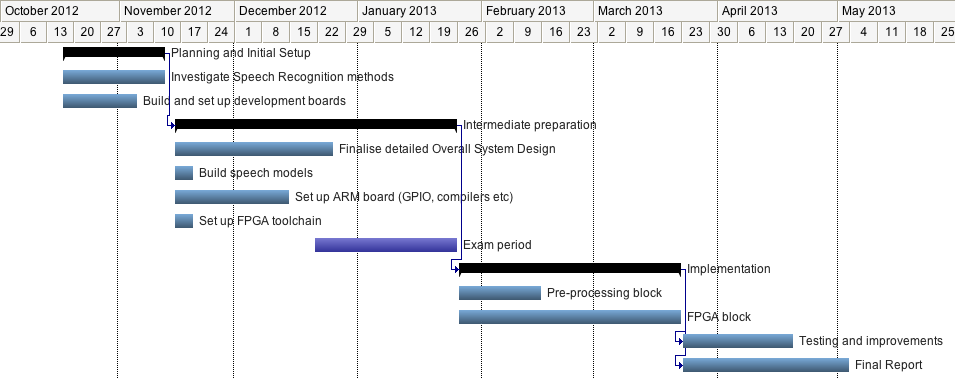
\includegraphics[width=\textwidth]{gantt-chart-initial.png}
	\end{center}
	\caption{First Gantt chart with high expectations}
	\label{fig:gantt1}
\end{figure}

\begin{figure}[tb]
	\begin{center}
		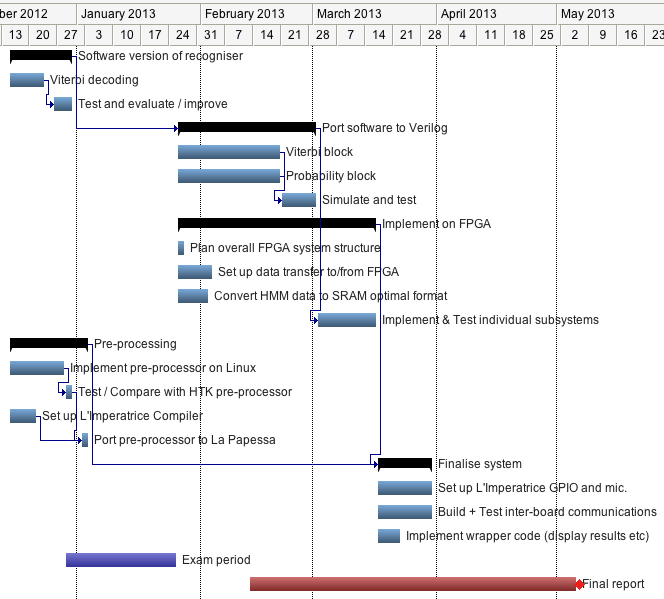
\includegraphics[width=\textwidth]{gantt-chart-interim.png}
	\end{center}
	\caption{Interim Gantt chart for remaining work}
	\label{fig:gantt2}
\end{figure}
% section overview (end)


\section{Details of tasks} % (fold)
\label{sec:details_of_tasks}
The implementation of the speech recogniser
% section details_of_tasks (end)


% chapter plan_of_remaining_work (end)